\chapter{轴突的生长和引导} \label{chap:chap47}


在前两章中,我们看到了神经元是如何在正确的时间和正确的位置以适当的数量生成。
这些早期发育步骤为后来的事件奠定了基础,这些事件指导神经元与目标细胞形成功能性联系。
为了形成连接,神经元必须延伸较长的过程(轴突和树突),它们允许与突触后细胞连接,并且可以从其他神经元接收突触输入。
在本章中,我们将研究神经元如何生成轴突和树突,以及轴突如何被引导至它们的目标。


本章首先讨论某些神经元突起成为轴突和其他树突的过程。
然后我们描述了生长中的轴突,它可能必须经过很长的距离并忽略许多不合适的神经元伙伴,然后才能在正确的区域终止并识别其正确的突触目标。
我们考虑了轴突克服这些挑战的策略。
最后,我们通过描述两个经过充分研究的轴突通路的发育来说明轴突引导的一般特征:
一个将视觉信息从视网膜传递到大脑,另一个将皮肤感觉信息从脊髓传递到大脑。



\section{轴突和树突之间的差异在发育早期就出现了}

\textit{神经元突起}在长度、厚度、分支模式和分子结构方面差异很大。
尽管如此,大多数神经元突起可以归入两个功能类别:轴突和树突。
一个多世纪以前,\textit{圣地亚哥$\cdot$拉蒙$\cdot$卡哈尔}假设这种区分是神经元向特定方向传输信息的能力的基础,他将这一想法形式化为\textit{动态极化理论}。
\textit{卡哈尔}写道,“神经冲动的传递总是从树突分支和细胞体到轴突。” 
在电生理学方法能够胜任这项任务之前的几十年里,这条定律提供了一种从组织学分析神经回路的方法。
尽管存在一些例外情况,但\textit{拉蒙$\cdot$卡哈尔}定律仍然一个基本原理,它将神经系统中的结构与功能联系起来,并强调了解神经元如何获得极化形态的重要性。


对神经元极化发生机制理解的进步,在很大程度上来自于对从啮齿动物大脑中提取并在组织培养中生长神经元的研究。
如图~\ref{fig:47_1}A~所示,在隔离条件下培养的海马神经元会发展出与活体内观察到的相似突起:一个单一的、长的、圆柱形的轴突和几个较短的、锥形的树突。
由于细胞骨架和突触蛋白以不同方式靶向这些成分,因此轴突和树突获得了独特的分子特征。
例如,如图~\ref{fig:47_1}B~所示,一种特定形式的\textit{微管相关蛋白}位于轴突中,\textit{微管相关蛋白}2 位于树突中。


\begin{figure}[htbp]
	\centering
	\includegraphics[width=0.91\linewidth]{chap47/fig_47_1}
	\caption{轴突和树突的分化标志着神经元极性的出现。
		A. 在组织培养中生长的海马神经元极化的四个阶段\cite{kaech2006culturing}。
		B. 在培养物中生长的海马神经元具有多个短而粗的树突,这些树突富含\textit{微管相关蛋白}2。
		它们还拥有一个长轴突,其特征是微管相关蛋白 tau 的去磷酸化形式(左)。
		从突变小鼠中分离出的培养神经元缺乏 Par 家族基因(SAD 激酶)的表达。
		神经元生成的神经突同时表达 tau 和 \textit{微管相关蛋白}2,分别是轴突和树突的标记。
		这些突起的长度和直径介于轴突和树突之间(右)\cite{kishi2005mammalian}。}
	\label{fig:47_1}
\end{figure}


培养的神经元对于发育研究特别有用,因为它们最初没有显示出明显的极化迹象,并在固定的细胞步骤序列中逐渐获得它们的专门特征。
这个序列从几个短的突起的延伸开始,每个突起在开始时都相当于其他突起。
如图~\ref{fig:47_1}A~所示,此后不久,其中一个突起形成轴突,其余突起获得树突特征。


% How does this occur? Cytoskeletal proteins
这是怎么发生的?
维持延伸过程和驱动生长的细胞骨架蛋白是这一过程的核心。
如果早期神经突中的肌动蛋白丝不稳定,细胞骨架就会重新配置,使神经突变成轴突;
其次,剩余的神经突反应成为树突。
如果新生的轴突被移除,剩余的神经突之一很快就会呈现出轴突特性。
该序列表明,轴突的特化是神经元极化的关键事件,并且新形成的轴突发出的信号既抑制了额外轴突的生成,也促进了树突的形成。


抑制其他轴突的轴突衍生信号的性质尚不清楚,但对于控制细胞骨架排列的信号,通过对Par复合体基因编码的一组蛋白的研究获得了一些见解。
正如在秀丽隐杆线虫中首次显示的那样,Par 蛋白参与细胞骨架重组的多个方面,包括神经元突起的极化。
如图~\ref{fig:47_1}B~所示,哺乳动物前脑神经元缺乏 Par 3、Par 4、Par 6或Par 1的亲缘蛋白,它们会长出多个长度介于轴突和树突之间的突起,并带有两个突起的标记。


尽管在培养物中生长的神经元与大脑中的神经元相似,但它们缺乏关键的外部线索和信号。
如图~\ref{fig:47_2}A~所示,培养的神经元彼此随机排列,而在发育中的大脑的许多区域,神经元排成一行,它们的树突指向同一方向。
随着神经元迁移到它们的目的地(第~\ref{chap:chap46}~章),轴突和树突通常分别作为它们的尾突和前导突的延伸而生长。
这种体内和体外的差异意味着外部信号调节极化机制。
如图~\ref{fig:47_2}C~所示,在发育中的大脑中,信号素和其他轴突引导因子的局部释放(本章后面将讨论)可能有助于树突的定向。
Par 蛋白复合物的作用是将这些细胞外信号与重新排列细胞骨架的细胞机制联系起来,这一过程部分是通过调节改变肌动蛋白或微管蛋白功能的蛋白质来实现的。
事实上,轴突中的\textit{微管相关蛋白}和树突中的 \textit{微管相关蛋白}2 蛋白都与微管相关并影响微管。
细胞骨架的差异也有助于放大轴突和树突之间区别的其他机制,例如分子的极化运输和轴突中特化初始片段的产生。


\begin{figure}[htbp]
	\centering
	\includegraphics[width=0.91\linewidth]{chap47/fig_47_2}
	\caption{细胞外因素决定神经元突起变成轴突还是树突。
		A. 体内大脑皮层锥体神经元显示出共同的轴突和树突方向。
		B. 在层粘连蛋白上生长的神经元获得极性。
		当一个皮层神经元从一个较不吸引人的基质上延伸出一个突起到层粘连蛋白上时,这个突起生长得更快,并且通常成为一个轴突。
		C. 在发育的新皮层中,软脑膜表面附近的细胞分泌\textit{信号素}-3A。
		\textit{信号素}-3A 是树突生长的引诱剂,有助于建立神经元极性和方向。
		在缺乏功能性\textit{信号素}-3A 的突变小鼠中,皮层锥体神经元的平行方向被破坏。}
	\label{fig:47_2}
\end{figure}


如果需要局部信号来极化大脑中的神经元,那么如何在组织培养的统一环境中建立极性?
一种可能的解释是,神经元内部信号强度的微小变化,或来自其直接环境的微小信号变化,将激活神经元一个小区域中的 Par 蛋白,使最近的细胞突起成为轴突。
如图~\ref{fig:47_2}B~所示,如果偶然,一个突起比它的邻居生长得稍微快一点,或者遇到一个加速神经突延伸的环境,它成为轴突的可能性显著增加。
据推测,这种原轴突突起发出的信号会降低其他突起效仿成为轴突的可能性,迫使它们变成树突。



\section{树突的形成受到内在因素和外在因素的共同影响}

一旦发生极化,树突就会生长和成熟,获得将它们与轴突区分开来的结构特征。
新生树突形成分支状的树状结构,其分支通常比轴突的分支更多,更靠近细胞体。
此外,许多树突的远端分支上会伸出称为棘的小突起。
最后,如图~\ref{fig:47_3}~所示,一些树突状分支被缩回或被“修剪”,以赋予树状结构其最终和确定的形状。


\begin{figure}[htbp]
	\centering
	\includegraphics[width=1.0\linewidth]{chap47/fig_47_3}
	\caption{树突分支按一系列步骤发育。
		树突的外生长涉及从其主干形成复杂的分支,随后在这些分支上发育出棘。
		在成熟的过程中,某些分支和棘会被修剪掉,以达到成熟的树突树状结构模式。}
	\label{fig:47_3}
\end{figure}


% Although the core features of dendrite formation
尽管树突形成的核心特征对于许多神经元来说是共同的,但不同类型的神经元在它们的数量、形状和分支模式上存在显著差异。
事实上,树突分支的形状是神经元分类的主要方式之一。
只需观察树突的模式,即可将小脑浦肯野细胞与颗粒细胞、脊髓运动神经元和海马锥体神经元区分开来。
这些差异对于不同类型神经元的不同功能至关重要。
例如,树突分支的大小及其分支的密度是其接收的突触数量的主要决定因素。


% How is dendritic pattern established? Neurons
树枝状模式是如何建立的?
如图~\ref{fig:47_4}~所示,神经元必须具有关于其形状的内在信息,因为组织培养中的模式与体内的模式非常相似。
指定神经元亚型的转录程序(第~\ref{chap:chap46}~章)可能也编码有关神经元形状的信息。
在无脊椎动物和脊椎动物中,一些转录因子由特定类型的神经元选择性地表达,并且似乎专门用于控制它们树突分支的大小、形状和复杂性。
这些转录因子通过协调下游基因的表达来实现这一目标,包括编码细胞骨架组件和介导与邻近细胞相互作用的膜蛋白的基因。


\begin{figure}[htbp]
	\centering
	\includegraphics[width=0.82\linewidth]{chap47/fig_47_4}
	\caption{神经元的形态保存在分离的细胞培养物中。
		小脑浦肯野神经元和海马锥体神经元具有独特的树突分支模式。
		当分离这两类神经元并在分离的细胞培养物中生长时,这些基本模式会被重新展现。}
	\label{fig:47_4}
\end{figure}


建立树突分支模式的第二种机制是同一细胞的其他树突识别某一个树突。
如图~\ref{fig:47_5}A~所示,在一些神经元中,树突彼此均匀分布,这种排列使它们能够有效地对输入进行采样,而不会出现大的间隙或团块。
在许多情况下,这种过程,称为自我回避,是通过一种机制发生的,即属于同一神经元的分支相互排斥。
如图~\ref{fig:47_5}D~所示,现已发现几种细胞表面粘附分子通过以导致排斥的方式相互作用来介导自我回避。
尽管相邻膜之间的粘附相互作用会导致排斥而不是附着似乎违反直觉,但大多数细胞间相互作用的结果是由它们发起的信号决定,而不是由粘附本身决定,正如我们将在本章后面看到的那样。


\begin{figure}[htbp]
	\centering
	\includegraphics[width=1.0\linewidth]{chap47/fig_47_5}
	\caption{树突分支之间的相互作用形成树突树状结构。
		A. 兄弟树突之间的自我回避导致分支的间距均匀,最大限度地减少间隙和团块。
		在视网膜\textit{星形无长突细胞}中,当伽马原钙粘蛋白丢失时,自我回避就会失败。
		B. 树突的平铺在概念上类似于自我回避,但适用于神经元群。
		它确保单一类型的相邻神经元有效地覆盖区域。
		C. 自我/非自我区分允许兄弟树突相互回避,同时可以自由地与其他相同类型神经元的树突进行相互作用。
		D. 通过在小鼠成簇\textit{原钙粘蛋白}位点(左)选择启动子和在果蝇 DSCAM1 位点(右)进行选择性剪接,从单个基因组复合体生成大量粘附分子。}
	\label{fig:47_5}
\end{figure}


邻近神经元的树突也提供线索。
如图~\ref{fig:47_5}B~所示,在许多情况下,特定类型神经元的树突以最小重叠覆盖表面,这种排列模式称为平铺。
树突的平铺在概念上与自我回避有关,但在平铺中,抑制性树突相互作用发生在特定类型的神经元之间,而在自我回避中,它们发生在单个神经元的兄弟树突之间。
平铺允许每种类型神经元接收其支配的整个表面或区域的信息。
通过一类神经元的树突对某个区域进行平铺还可以避免由于许多不同神经元的树突占据同一区域而可能产生的混淆。


% A particularly interesting situation is one in
一个特别有趣的情况是,树突进行自我回避,但与其他同类细胞的树突形成突触。
如图~\ref{fig:47_5}C~所示,在这种情况下,树突面临着一个挑战性的任务:它们需要区分本质上相同的树突,即来自本质上相同的细胞的树突。
已经确定了两组介导这种自我/非自我辨别的分子:哺乳动物中的成簇原钙粘蛋白和果蝇中的 DS-CAM。
如图~\ref{fig:47_5}D~所示,尽管它们在结构上不相关,但它们有几个共同特征。


% First, both are encoded by large, complex genes
首先,两者都由产生大量同源异构体的大型复杂基因编码。
果蝇 Dscam1 基因通过选择性剪接能够编码大约 3 万 8 千种不同的蛋白质,而集簇性原钙粘蛋白编码大约 60 种蛋白质,这些蛋白质可以组装成数千种不同的多聚体。
其次,几乎所有的异构体都同亲型结合;
例如,一个树突表面上的原钙粘蛋白 $\gamma$a1 与相邻膜上的原钙粘蛋白 $\gamma$a1 结合良好,但与其他异构体的结合很差或者根本无法结合。
第三,每个神经元在其群体中以一种尚不完全理解的方式表达所有可能的Dscam1或原钙粘蛋白异构体的随机子集。
鉴于异构体数量庞大,单个神经元在其细胞表面表达相同的异构体集合的可能性很小。
结果是,每个神经元的树突通过同型结合与同源树突发生相互作用,导致排斥和自我回避,而与邻近神经元的树突结合较差,这使得其他识别系统能够促进突触形成。


总之,我们所描述的机制以及许多其他机制,通过内在机制和细胞外机制的结合,建立了整体的分支模式。
对于树突,外在模式信号决定了神经元的形态。
对于我们接下来要考虑的轴突,信号引导轴突到达它们的目标。



\section{生长锥是一种感觉传感器和运动结构}

一旦轴突形成,它就开始向其突触目标生长。
负责轴突生长的关键神经元元素是轴突尖端的一种特殊结构,称为生长锥。
轴突和树突都使用生长锥来伸长,但与轴突相关的生长锥已得到更深入的研究。


如图~\ref{fig:47_6}A~所示,\textit{拉蒙$\cdot$卡哈尔}发现了生长锥,并且具有关键的洞察力,认为生长锥负责轴突的路径寻找。
仅以静态图像作为灵感,他设想生长锥“具有精湛的化学敏感性、快速的变形虫运动和一定的动力,因此它能够继续前进并克服途中遇到的障碍……直到到达目的地。”


\begin{figure}[htbp]
	\centering
	\includegraphics[width=1.0\linewidth]{chap47/fig_47_6}
	\caption{神经元生长锥。
		A. \textit{圣地亚哥$\cdot$拉蒙$\cdot$卡哈尔}绘制的生长锥图,他发现了这些细胞结构并推断了它们的功能。
		B. 在小鼠视网膜神经节细胞中,通过染色标记可视化的生长锥。
		请注意与卡哈尔绘图的相似之处。
		C. 通过整体扫描电子显微镜显示的生长锥的 3 个主要区域:丝状伪足、片状伪足和中央核。
		D. 来自海兔的神经元的生长锥,其中肌动蛋白和微管蛋白已经显现。
		肌动蛋白(紫色)集中在片状伪足和丝状伪足中,而微管蛋白和微管(天蓝色)集中在中央核。}
	\label{fig:47_6}
\end{figure}


过去一个世纪的许多研究证实了\textit{拉蒙$\cdot$卡哈尔}的直觉。
我们现在知道,生长锥既是一个感觉结构,接收来自环境的方向性线索,也是一个运动结构,其活动驱动轴突延长。
\textit{拉蒙$\cdot$卡哈尔}还思考了“在这些过程出现之前有哪些神秘力量……促进它们的生长和分支。
并最终建立起那些原生质之吻。
这似乎构成了一个史诗般爱情故事的最后狂喜。” 
用更现代和通俗的话来说,我们现在知道生长锥通过将正负信号转变成调节细胞骨架的信号来引导轴突,从而确定轴突向其目标生长的过程和速度,它将在此处形成突触。


生长锥具有 3 个主要的区域。
它们的中央核富含微管、线粒体和其他细胞器。
从生长锥体伸出称为丝状伪足的细长延伸物。
如图~\ref{fig:47_6}C、D~所示,丝状伪足之间是片状伪足,它们也能运动,并赋予生长锥特有的褶皱外观。


生长锥体通过它们的丝状伪足感知环境信号:这些丝状伪足是棒状的、富含肌动蛋白、限定在膜内的结构,具有高度的移动性。
它们的表面膜带有受体,这些受体充当轴突的定向信号。
丝状伪足的长度(在某些情况下可达数十微米)使他们能够在生长锥的中央核之前对环境进行采样。
它们的快速移动使它们能够详细记录环境信息,它们的灵活性使它们能够绕过细胞和其他障碍物进行导航。


当丝状伪足遇到环境中的信号时,生长锥会受到刺激前进、后退或转向。
有几个动力来源驱动这些定向行为。
其中一种动力来源是肌动蛋白沿肌球蛋白的运动,这种相互作用与驱动骨骼肌纤维收缩的过程类似,尽管神经元的肌动蛋白和肌球蛋白与肌肉中的不同。
肌动蛋白单体组装成聚合物丝也有提供了丝状伪足延伸的推进力。
由于肌动蛋白丝在丝状伪足的基部不断解聚,聚合和解聚的平衡使丝状伪足向前移动而不会变长。
在生长锥前进期间,解聚减慢,导致更大的净向前运动。
膜沿基底的运动提供了另一种向前运动的动力来源。


% The contribution of each type of molecular
每种类型的分子马达对生长锥推进的贡献可能因情况而异。
然而,最后一步涉及微管从生长锥的中央核流入新延伸的尖端,从而使生长锥向前移动并在其后留下新的轴突片段。
如图~\ref{fig:47_7}~所示,在前进的生长锥中形成新的\textit{板状伪足}和\textit{线状伪足},然后这个循环重复进行。


\begin{figure}[htbp]
	\centering
	\includegraphics[width=1.0\linewidth]{chap47/fig_47_7}
	\caption{生长锥在细胞马达的控制下前进\cite{heidemann1996cytoplasmic}。
		A. 丝状伪足接触粘附信号并发生收缩,从而向前拉动生长锥(1)。
		肌动蛋白丝在丝状伪足的前缘聚集,在后缘解聚,在此过程中与肌球蛋白相互作用(2)。
		肌动蛋白聚合推动丝状伪足向前(3)。
		肌动蛋白逆行产生的力推动丝状伪足向前。
		胞吐作用将膜添加到丝状足的前缘,并提供新的粘附受体以保持牵引力。
		在丝状足的背面回收膜。
		肌动蛋白聚合物与质膜上的粘附分子相连。
		B. 这些马达的联合作用创造了一个肌动蛋白耗尽的空间,该空间由来自中心核心的微管前进填充。
		C. 单个微管凝聚成一个粗束,细胞质围绕它们塌陷,形成新的轴突段。}
	\label{fig:47_7}
\end{figure}


只有当生长锥的运动动作与其感觉功能相关联时,才能进行准确的寻路。
因此,至关重要的是,丝状伪足上的识别蛋白是信号诱导受体,而不仅仅是介导粘附的结合部分。
配体与其受体的结合以多种方式影响生长。
如图~\ref{fig:47_7}~所示,在某些情况下,它通过受体的细胞内结构域直接与细胞骨架结合。
当整合素受体结合邻近细胞表面的分子或细胞外基质时,它们与生长锥中的肌动蛋白相连,从而影响运动性。


同样重要甚至更重要的是配体结合刺激作为第二信使发挥作用的可溶性细胞内分子的形成、积累甚至分解的能力。
这些第二信使影响细胞骨架的组织,并以此方式调节生长锥运动的方向和速度。


一个重要的第二信使是钙。
生长锥中的钙浓度受丝状伪足上受体激活的调节,这会影响细胞骨架的组织,进而调节运动性。
生长锥的运动性在一种称为设定点的钙浓度狭窄范围内最佳。
生长锥一侧的丝状伪足的激活导致整个生长锥的钙浓度梯度的形成,为生长方向的变化提供了可能的基础。


其他将受体与运动分子联系起来的第二信使包括环状核苷酸,它们调节诸如蛋白激酶、蛋白磷酸酶和 rho 家族\textit{三磷酸鸟苷}酶的活性。
反过来,这些信使和酶调节控制肌动蛋白丝聚合和解聚的蛋白质的活性,从而促进或抑制轴突延伸。


细胞内信号在生长锥运动和方向中的关键作用可以通过在培养物中生长的胚胎神经元来证明。
将生长因子应用于生长锥的一侧会激活局部受体,并导致生长锥向信号源延伸和转向。
本质上,生长因子吸引了生长锥。
然而,如图~\ref{fig:47_8}A~所示,当神经元中的\textit{环磷酸腺苷}水平降低时,相同的刺激会变成排斥信号,并且生长锥会远离信号。
当第二信使\textit{环鸟苷-3,5-单磷酸盐}的水平升高时,其他排斥因素可能变得有吸引力。


\begin{figure}[htbp]
	\centering
	\includegraphics[width=1.0\linewidth]{chap47/fig_47_8}
	\caption{细胞内调节蛋白水平的变化可以决定生长锥对同一外在导向信号是吸引还是排斥。
		A. \textit{蛋白激酶A}的活性状态可以改变生长锥对细胞外定向因子的反应,在本例中为蛋白质\textit{轴突导向因子}。
		当\textit{蛋白激酶A}活性和细胞内\textit{环磷酸腺苷}水平较低时,生长锥会被 \textit{轴突导向因子}排斥。
		当\textit{蛋白激酶A}活性高时,细胞内\textit{环磷酸腺苷}的升高导致生长锥吸引局部\textit{轴突导向因子}源\cite{ming1997camp}。
		B. 生长锥受体的\textit{轴突导向因子}激活(在\textit{结直肠癌缺失蛋白}中缺失)导致肌动蛋白的局部合成,从而导致转向。
		C. 生长锥的免疫组织化学分析显示,局部应用\textit{轴突导向因子}会引起局部肌动蛋白的合成反应\cite{leung2006asymmetrical} }
	\label{fig:47_8}
\end{figure}


最近,另一种将导向分子与生长锥行为耦合的机制已经显现出来。
长期以来,人们认为所有神经元蛋白质的合成都发生在细胞体中,但我们现在知道,生长锥(以及一些树突)含有蛋白质合成机制,包括一部分\textit{信使核糖核酸}。
这些分子发挥重要作用的初步证据来自轴突与母细胞体分离的实验。
生长锥继续前进了几个小时; 它们可以被刺激转向或远离局部的引导分子的局部存储库,而这些行为被蛋白质合成抑制剂所消除。
如图~\ref{fig:47_8}~所示,局部蛋白质合成是由生长锥上导向受体激活产生的第二信使调节。
这种机制导致在需要的时间和地点精确地合成新的运动蛋白。
因此,生长锥有许多策略和机制来整合分子信号,以指导轴突向特定方向前进。



\section{分子线索引导轴突到达目标}

在 20 世纪的大部分时间里,关于生长锥如何通过胚胎地形到达目标的两种截然不同观点的倡导者之间展开了激烈的辩论。
20 世纪之交,生理学家\textit{兰列}首次阐述了轴突导向的分子观点。
但到了 1930 年代,包括\textit{保罗$\cdot$韦斯}在内的许多著名生物学家认为,轴突的生长本质上是随机的,适当的连接主要因为轴突及其目标细胞中有成效的、匹配的电活动模式而得以维持。


在我们的分子时代,\textit{韦斯}的想法看似简单,但在当时并非没有道理。
在组织培养中,轴突优先沿着机械不连续点(盖玻片上的划痕和凸起)生长,胚胎神经干通常与固体支撑物(血管或软骨)对齐。
\textit{韦斯}认为机械引导(称为立体定向)可以解释轴突模式,这似乎是合乎逻辑的。
今天,我们非常习惯于这样的想法:电信号可以被用来改变计算机中电流的流动,而无需重新焊接连接。
同样,活动模式和经验可以加强或削弱神经连接,而不需要形成新的轴突通路。
那么,为什么不考虑建立适当联系所涉及的一致活动(\textit{韦斯}称之为共振)呢?


今天,很少有科学家认为立体定向或共振是神经回路初始模式形成的关键力量。
使观点转向支持分子观点的转折点是 1940 年代\textit{罗杰$\cdot$斯佩里}(具有讽刺意味的是,他是\textit{韦斯}的学生)用青蛙和其他两栖动物进行的实验。
\textit{斯佩里}操纵由视网膜神经节细胞的轴突从眼睛传送到大脑的信息。
这些轴突终止于它们的目标区域,丘脑中的外侧膝状体和中脑中的上丘(在低等脊椎动物中称为视顶盖),以这样一种方式创建了有序的视野\textit{视网膜映射}。


% Because of the optics of the eye, the
由于眼睛的光学特性,视网膜上的视觉图像是视野的倒像。
如图~\ref{fig:47_9}A~所示,视网膜神经节细胞通过其轴突终止于视顶盖(青蛙大脑中的主要视觉中心)的模式重新反转图像。
如果视神经被切断,动物就会失明。
在低等脊椎动物中,切断的视网膜轴突可以重新建立对顶盖的投射,从而恢复视觉。
哺乳动物的情况并非如此,我们将在第~\ref{chap:chap50}~章中讨论。


\begin{figure}[htbp]
	\centering
	\includegraphics[width=1.0\linewidth]{chap47/fig_47_9}
	\caption{\textit{罗杰$\cdot$斯佩里}关于视觉系统再生的经典实验为连接线路中的化学亲和力提供了证据。
		A. 在青蛙的视觉系统中,晶状体将倒置的视觉图像投射到视网膜上,然后视神经将图像连同额外的倒置一起传输到视顶盖。
		视网膜输入到视顶盖的空间排列允许这种转移。
		前视网膜中的神经元将轴突投射到后顶盖,而后视网膜中的神经元投射到前顶盖。
		同样,背侧视网膜中的神经元投射到腹侧顶盖,而腹侧视网膜中的神经元投射到背侧顶盖。
		因此,视觉引导的行为(这里是抓苍蝇)是准确的。
		B. 如果视神经被切断,并且在神经再生之前通过手术将眼睛在其眼窝中旋转,视觉引导的行为就会异常。
		当一只苍蝇出现在头顶时,青蛙会将其感知为下方,反之亦然。
		行为反射的倒置是由再生的视网膜轴突与其原始目标的连接引起的,尽管这些连接现在将一个倒置的、不合适的世界映射传输到大脑中。}
	\label{fig:47_9}
\end{figure}


\textit{斯佩里}的关键实验是切断青蛙的视神经,然后在神经再生之前将眼球在眼窝中旋转 180°。
值得注意的是,这只青蛙对视觉输入表现出了有序的反应,但这种行为是错误的。
如图~\ref{fig:47_9}B~所示,当青蛙在地上看到一只苍蝇时,它会跳起来,当在它头顶上方有一只苍蝇时,它会向下击打。
重要的是,这种动物从未学会改正错误。
\textit{斯佩里}提出:后来用解剖学和生理学方法证实,视网膜轴突重新支配了它们原来的顶盖目标,尽管这些连接为大脑提供了导致异常行为的错误空间信息。
这些实验的推论是,轴突及其目标之间的识别依赖于分子匹配,而不是随机连接的功能验证和改进。


% But Weiss’s ideas are by no means obsolete.
但\textit{韦斯}的想法绝不会过时。
事实上,我们现在认识到神经回路的活动可以在塑造连通性方面发挥关键作用。
目前的观点是,分子匹配在胚胎发育过程中占主导地位,而活动和经验会在回路形成后对其进行修改。
在本章和下一章中,我们描述了指导神经连接形成的分子线索,然后在第~\ref{chap:chap49}~章中,我们研究了活动和经验在微调突触连接中的作用。


\textit{斯佩里}的猜想,通常称为化学特异性假说,促使发育神经生物学家寻找轴突和突触“识别分子”。
在最初的几十年里,这方面的成功有限,部分原因是这些分子的数量很少,并且仅出现在离散的神经元子集上,同时缺乏有效的方法从复杂组织中分离出稀有分子。
最终,生物化学和分子生物学方法的进步使这项任务变得更加可行,并且现在已经发现了许多参与将轴突引导至其目标的蛋白质。
这些蛋白质通常由成对的配体和受体组成:配体由轴突沿途的细胞呈现,受体由生长锥本身呈现。


用最一般的术语来说,指导线索可以出现在细胞表面、细胞外基质中,或以可溶性形式存在。
如图~\ref{fig:47_8}~所示,它们与嵌入生长锥膜中的受体相互作用,以促进或抑制轴突的生长。
大多数受体都有一个胞外结构域,可以选择性地结合同源配体,以及一个胞内结构域,可以直接或通过第二信使等中间体与细胞骨架偶联。
配体可以加速或减缓生长。
出现在生长锥一侧的配体可导致局部激活或抑制,从而导致转向。
这样,环境线索的局部分布决定了前进的\textit{生长锥}通路。


如图~\ref{fig:47_10}~和~图~\ref{fig:47_11}~所示,由于这些最近的发现,轴突导向(一个多年前出现的神秘过程)现在可以被视为蛋白质-蛋白质相互作用的有序结果,它指导生长锥生长、转动、分岔或停止。
这一有限的指令集,当以空间精度呈现时,足以精心编排生长锥行为的微妙变化。
因此,可以通过描述配体的呈现方式和位置以及生长锥如何整合此信息以产生有序反应来解释轴突引导。
在本章的其余部分,我们通过描述两种类型的轴突旅程来说明所学到的经验教训:
视网膜神经节神经元的轴突和脊髓中特定类别的感觉中继神经元的轴突。



\section{视网膜神经节轴突的生长以一系列离散步骤为导向}

\textit{斯佩里}的实验暗示了轴突引导线索的存在,但没有揭示它们的位置或工作方式。
有一段时间,一个突出的观点是识别主要发生在目标处或附近,机械力或远程趋化因子足以使轴突到达目标附近。


我们现在知道,轴突通过一系列不连续的步骤到达远距离目标,沿着它们的路线以紧密的间隔做出频繁的决定。
为了说明这一点,我们将追踪\textit{斯佩里}试图理解的路径,即视网膜轴突生长到视顶盖的路径。



\subsection{生长锥在视交叉处发散}

视网膜神经节细胞轴突的首要任务是离开视网膜。
当它进入视神经纤维层时,它沿着视网膜边缘的基底膜和神经胶质末端延伸。
轴突的生长从一开始就是定向的,表明它可以读取环境中的定向线索。
如图~\ref{fig:47_12}~所示,当它接近视网膜中心时,它受到从视神经乳头(视神经与视网膜本身的连接处)发出的引诱剂的影响,引导它进入视柄。
然后它沿着视神经走向大脑。


\begin{figure}[htbp]
	\centering
	\includegraphics[width=1.0\linewidth]{chap47/fig_47_12}
	\caption{视网膜神经节细胞的轴突以不连续的步骤生长到视顶盖。
		图中显示了两个神经元,它们携带来自视网膜鼻侧的信息。
		一个神经元的轴突穿过视交叉到达对侧视顶盖。
		另一个神经元的轴突也穿过视交叉但投射到外侧膝状体核。
		这些数字表示轴突旅程中的重要地标。
		生长的轴突指向视神经乳头(神经与视网膜的连接处)(1),进入视神经(2),延伸穿过视神经(3),在视交叉处转向保持同侧(未显示)或交叉到对侧(4),延伸穿过视束(5),进入视顶盖或外侧膝状体核(未显示)(6),导航至适当的头尾侧和背腹侧位置(7),转向进入神经网(如图所示,在鸟类中下行;在哺乳动物中上行)(8),在适当的层级停下,形成原始的末端树突(9),最后进行重塑(10)。}
	\label{fig:47_12}
\end{figure}


沿着这条路线行进的第一个轴突跟随视茎细胞,视茎细胞是连接视网膜和它起源的间脑的神经管的雏形。
然后,这些“先锋”轴突充当后来到达轴突的支架,这些轴突只需跟随它们的前辈就能够准确地延伸(参见图~\ref{fig:47_10}~中的“束化”)。
然而,一旦它们到达视交叉,视网膜轴突就必须做出选择。
如图~\ref{fig:47_13}~A~所示,由每只眼睛的鼻侧视网膜中的神经元产生的轴突穿过视交叉并前进到大脑的另一侧,而来自颞半部的轴突在到达视交叉时发生偏转,因此停留在大脑的同一侧。


\begin{figure}[htbp]
	\centering
	\includegraphics[width=1.0\linewidth]{chap47/fig_47_13}
	\caption{视网膜神经节神经元的轴突在到达视交叉时发散。
		A. 延时系列显示轴突接近中线。
		源自鼻侧视网膜的轴突穿过视交叉并投射到对侧顶盖(左)。
		相比之下,来自颞侧视网膜的轴突到达视交叉但未能穿过,因此投射到同侧顶盖(右)。
		B. 自颞侧视网膜的神经元轴突表达酪氨酸激酶受体EphB1,当它们遇到在视交叉处表达ephrin-B2的中线放射状胶质细胞时,被阻止穿越中线。
		而鼻侧视网膜神经元的轴突缺乏EphB1受体,因此不受ephrin-B2的影响,能够穿越到对侧。
		C. 更高放大倍数的视图,展示了视网膜神经节细胞轴突在视交叉处的轨迹。}
	\label{fig:47_13}
\end{figure}


\begin{figure}[htbp]
	\centering
	\includegraphics[width=1.0\linewidth]{chap47/fig_47_10}
	\caption{细胞外线索使用多种机制来引导生长锥。
		轴突可以与细胞外基质中的生长促进分子相互作用(1)。
		它可以与神经细胞上的粘附细胞表面分子相互作用(2)。
		生长中的轴突会遇到来自“先锋”神经元的另一个轴突并沿着它移动,这一过程称为束化(3)。
		可溶性化学信号可以将生长的轴突吸引到其细胞源(4)。
		表达细胞表面排斥信号的中间靶细胞可导致轴突转向(5)。
		可溶性化学信号可以排斥生长中的轴突(6)。
		细胞外信号还导致从轴突轴形成侧支(7)或生长轴突的分支(8)。}
	\label{fig:47_10}
\end{figure}


这种轨迹的差异反映了来自鼻侧和颞侧视网膜的轴突对视交叉中线细胞呈现的引导线索的不同反应。
一些视网膜轴突接触并穿过视交叉细胞,而另一些则被这些细胞抑制并偏转,从而留在同侧。
如图~\ref{fig:47_13}B~所示,交叉细胞呈现的关键分子之一是 ephrin-B 家族的膜结合型排斥分子,它也出现在视网膜神经节细胞轴突导向的后续步骤中。


向同侧投射的颞叶视网膜轴突的比例因物种而异:
低等脊椎动物中很少,啮齿类动物中有一些,而人类中有很多。
这些差异反映了眼睛的位置。
在许多动物中,眼睛指向两侧并监测视觉世界的不同部分,因此不需要将两只眼睛的信息结合起来。
在人类中,双眼向前看,并且大部分视觉世界区域是重叠的,因此协调视觉输入是至关重要的。


穿过视交叉后,视网膜轴突沿着间脑腹侧表面在视束中聚集。
然后轴突在不同的点离开视束。
在大多数脊椎动物物种中,中脑的视顶盖(在哺乳动物中称为上丘)是视网膜轴突的主要目标,但少数轴突投射到丘脑的外侧膝状体核。
然而,在人类中,大多数轴突投射到外侧膝状体,相当多的轴突投射到上丘,小部分投射到枕核、视交叉上核和顶盖前核。
在这些目标中,不同的视网膜轴突投射到不同的区域。
正如\textit{斯佩里}所展示的,视网膜轴突在顶盖表面形成了精确的\textit{视网膜映射}。
在其他由视网膜轴突支配的区域(如外侧膝状体)也形成了类似的映射图。


到达顶盖内的适当位置后,视网膜轴突需要找到合适的突触伙伴。
如图~\ref{fig:47_12}~所示,为了完成他们旅程的最后阶段,视网膜轴突转向并进入顶盖神经细胞,沿着放射状神经胶质细胞表面下行(或者在哺乳动物中上行),这为放射状轴突生长提供了支架。
虽然放射状神经胶质细胞跨越神经上皮的整个范围,但每个视网膜轴突将其\textit{突触末稍}限制在单层。
许多突触后细胞的树突延伸穿过多层并沿其整个长度形成突触,但视网膜输入仅限于目标神经元树突树的一小部分。
这些组织特征意味着特定于层的线索会阻止轴突伸长并触发树枝化。


因此,长距离轴突导航的问题通过将旅程分成短段来解决,在这些短段中,中间目标引导轴突沿着路径到达最终目标。
一些中间目标(例如视交叉)是轴突发散的“决策”区域。


依靠中间目标是解决远距离轴突导航问题的有效方法,但不是唯一的方法。
在某些情况下,当胚胎较小且要覆盖的距离较短时,第一个轴突会到达它们的目标。
这些“先锋”轴突沿途对嵌入细胞或细胞外基质的分子信号作出响应。
第一个离开视网膜的轴突属于这一类。
稍后出现的轴突,当距离较长且障碍较多时,可以跟随先锋轴突到达它们的目标。
另一种引导机制是分子梯度。
事实上,正如我们将看到的,视顶盖中细胞表面分子的梯度会告知轴突其正确的终止区。



\subsection{\textit{轴突导向因子}的梯度在大脑中提供抑制信号}

到目前为止,我们已经了解了视网膜轴突如何通过响应一系列离散的方向线索来到达视顶盖。
然而,生长过程中的这些选择并不能解释\textit{斯佩里}对顶盖\textit{视网膜映射}的平滑分级连接的分析。
对假设的“映射分子”的探索成为发育神经生物学家的主要关注点,因此我们对其进行了一些详细描述。


随着生物测定的发展,对这些分子的探索取得了重大突破,其中来自视网膜特定部分的外植体被放置在由顶盖膜碎片组成的基质上。
膜碎片取自顶盖的明确前后部分,并以交替条纹的方式排列。 
如图~\ref{fig:47_14}~所示,研究发现,来自颞侧(后侧)半视网膜的轴突优先生长在来自前顶盖的膜上,这种偏好与体内表现出来的偏好相似。
这种偏好被发现是由于后膜中存在抑制因子,而不是前膜中有吸引或粘附物质引起的。
这一观察是首次证明抑制或排斥物质在轴突导向中的作用。


\begin{figure}[htbp]
	\centering
	\includegraphics[width=0.86\linewidth]{chap47/fig_47_14}
	\caption{排斥信号在体外指导视网膜轴突的发育。
		A. 来自后部(颞侧)半视网膜的视网膜神经节轴突投射到前部发育中的顶盖中。
		相反,来自前(鼻)半视网膜的轴突投射到后顶盖。
		B. 从视顶盖的特定前后部位取出的膜片段,并以交替条纹的方式排列。
		来自后部视网膜外植体的轴突选择性地生长在前顶盖的片段上。
		轴突在前膜上的优先生长是由后膜中的抑制信号引起。
		相反,来自前部视网膜的轴突在前部和后部视顶盖膜片段上都能生长\cite{walter1987avoidance}。}
	\label{fig:47_14}
\end{figure}


这种条纹测定允许表征抑制线索,存在于后顶盖的膜中而不是前顶盖。
分子生物学家独立地发现了受体酪氨酸激酶家族(即 Eph 激酶),以及膜相关配体大家族(ephrins)。
受体和配体都分为 A 亚族和 B 亚族。
ephrin-A 蛋白能结合并激活 EphA 激酶;
反之,如图~\ref{fig:47_11}C~所示,ephrin-B 蛋白能结合并激活 EphB 激酶。


\begin{figure}[htbp]
	\centering
	\includegraphics[width=0.85\linewidth]{chap47/fig_47_11}
	\caption{不同的分子家族控制发育中轴突的生长和导向。
		A. 大量经典钙粘蛋白家族主要通过相邻神经元上钙粘蛋白分子之间的同源相互作用促进细胞和轴突粘附。
		粘附相互作用是通过细胞外EC1结构域的相互作用介导。
		钙粘蛋白通过其与连环蛋白的细胞质相互作用来传导粘附相互作用,连环蛋白将钙粘蛋白与肌动蛋白细胞骨架连接起来。
		B. 多种免疫球蛋白超家族蛋白在神经系统中表达,并介导粘附相互作用。
		这里显示的 3 个例子 NCAM,L1和TAG1,可以通过同源和异源结合以促进轴突生长和粘附。
		这些蛋白质包含免疫球蛋白结构域(圆形)和纤维连接蛋白III型结构域(方形)。
		同源相互作用通常涉及氨基末端免疫球蛋白结构域。
		不同的免疫球蛋白粘附分子通过不同的细胞质介质与细胞骨架相互作用,此处仅显示其中的少数。
		C. 不同的ephrin蛋白与Eph类酪氨酸激酶受体结合。
		A类ephrin通过糖基磷脂酰肌醇系链与表面膜连接,而B类ephrin是跨膜蛋白。
		A类ephrin通常与A类Eph激酶结合,B类ephrin通常与B类Eph激酶结合。
		正向Eph信号传导通常在接受细胞中引起排斥或抑制反应,而反向ephrin信号传导可引起粘附或抑制反应。
		Ephrin-Eph信号传导涉及许多不同的细胞质介质。
		D. 层粘连蛋白是细胞外基质的组成部分,通过与整合素受体的相互作用促进细胞粘附和轴突延伸。
		整合素通过许多中间蛋白与细胞骨架相互作用介导粘附和轴突生长。
		E. 信号蛋白可以通过与多种丛蛋白和神经毡蛋白受体相互作用来促进或抑制轴突生长,这些受体通过Rho类\textit{三磷酸鸟苷}酶和下游激酶传导信号。
		F. Slit蛋白通常通过与Robo类受体的相互作用介导排斥反应,这些受体通过\textit{三磷酸鸟苷}酶,如Rac影响轴突生长。
		G. 分泌的或与细胞外基质相关的\textit{轴突导向因子}蛋白介导化学引诱和化学排斥反应。
		\textit{引诱反应}是通过与\textit{结直肠癌缺失蛋白}受体的相互作用介导的,而排斥反应涉及与\textit{结直肠癌缺失蛋白}和unc-5辅助受体的相互作用。
		\textit{轴突导向因子}受体通过GTPases和\textit{环鸟苷-3,5-单磷酸盐}级联发出信号。}
	\label{fig:47_11}
\end{figure}


当视顶盖抑制信号被确定为 ephrin-A5 时,这两条研究领域汇聚在一起。
我们现在知道,Eph 激酶和ephrins在神经和非神经组织中发挥多种功能,并且每一类蛋白质都可以根据细胞环境的不同,作为配体或受体。
在发育中的神经系统中,这些蛋白质构成了主要的排斥信号组。


Ephrin-Eph 相互作用在很大程度上解释了顶盖中\textit{视网膜映射}的形成。
顶盖中肝配蛋白-A2 和肝配蛋白-A5 的水平以及视网膜中 Eph 受体的水平沿前后轴呈阶梯分布。
这些梯度方向相同。
如图~\ref{fig:47_15}A~所示,Ephrin-A 浓度在顶盖中从后高到前低,而 Eph A 浓度在视网膜中从后高到前低。
这种反梯度至少部分地解释了地形映射。
来自后部视网膜神经节细胞的轴突,其EphA受体水平较高,会被后部视顶盖中高水平的ephrin-A强烈排斥,因此被限制在前部视顶盖。
来自前部视网膜不太敏感的轴突能够进一步穿透到顶盖的后部区域。
因此肝配蛋白-A2 和肝配蛋白-A5 是\textit{斯佩里}假设的化学特异性因子的有力候选者。


\begin{figure}[htbp]
	\centering
	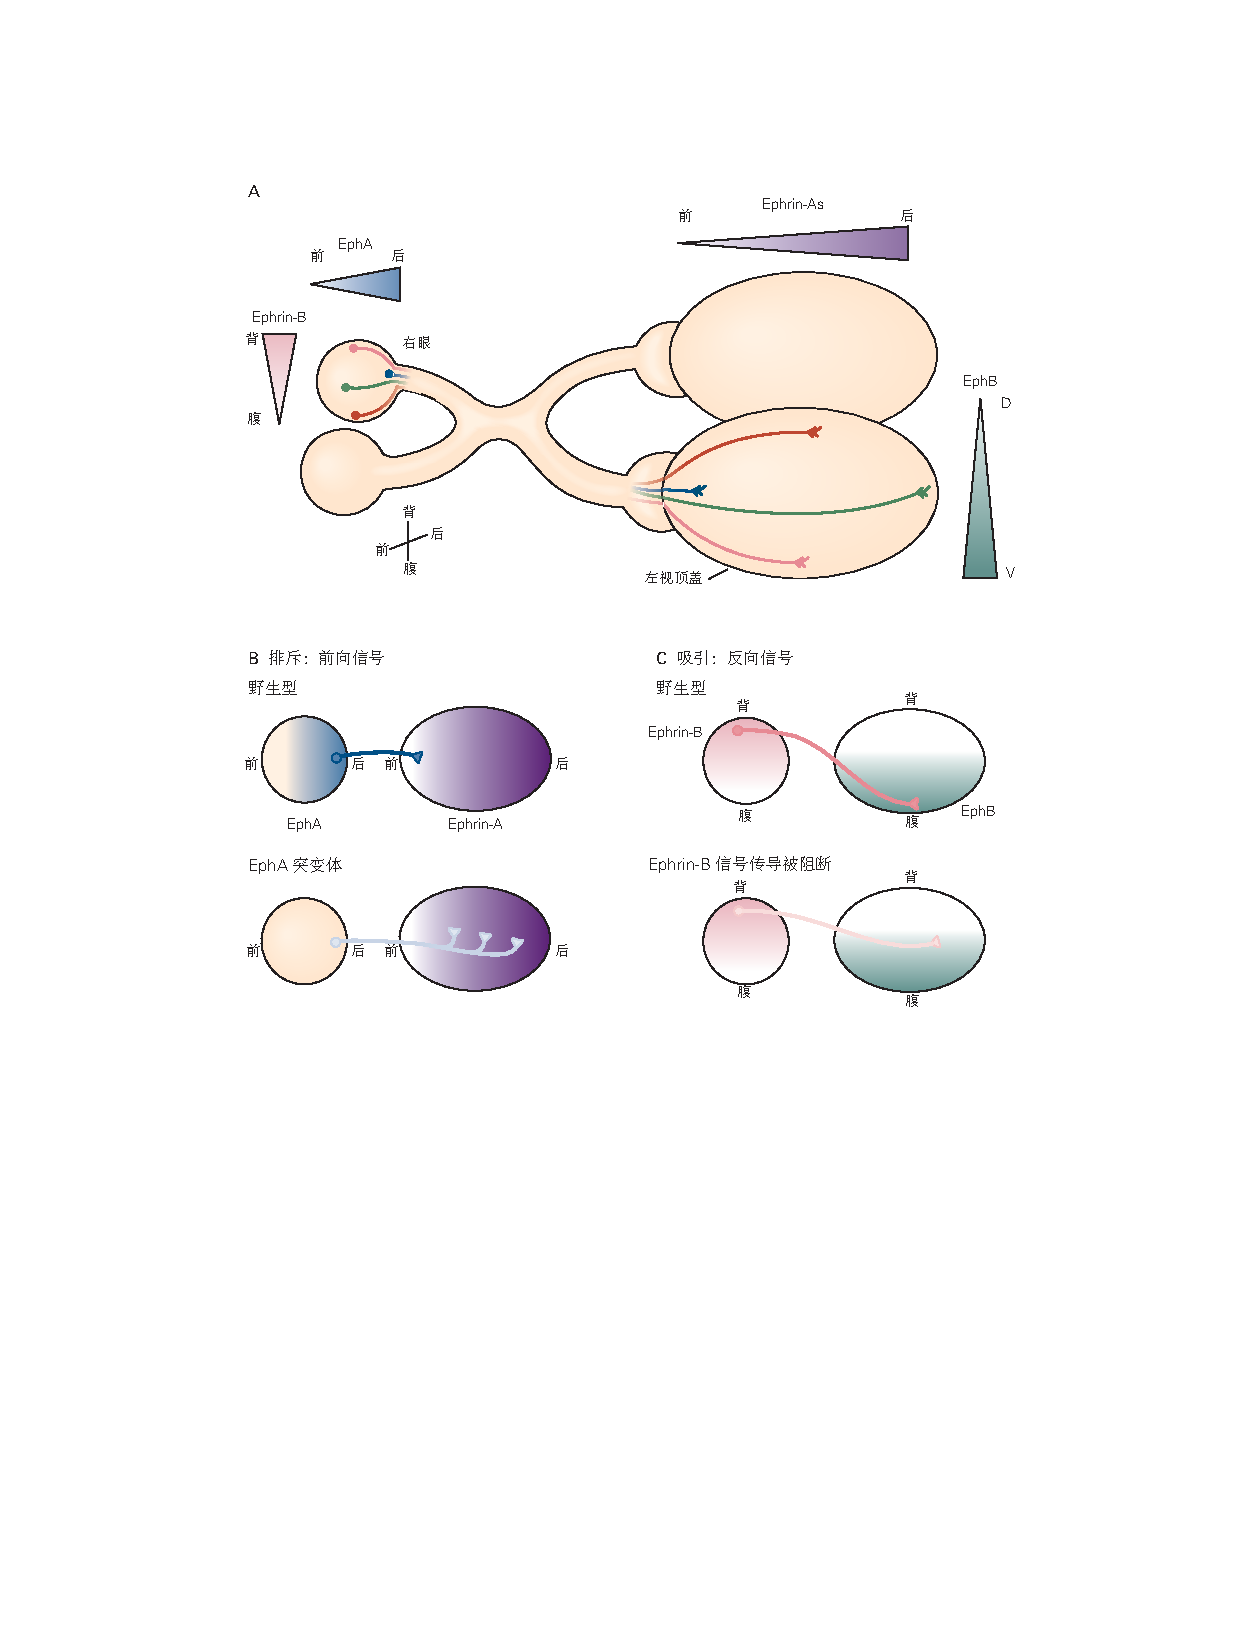
\includegraphics[width=0.85\linewidth]{chap47/fig_47_15}
	\caption{体内\textit{视网膜映射}的形成取决于 ephrin-Eph 激酶信号。
		A. 在视网膜中,EphA 受体以\textit{前后}梯度表达,ephrin-B 以\textit{背腹}梯度表达。
		在顶盖中,ephrin-A 受体呈前后梯度分布,EphB 呈背腹梯度分布。
		B. EphA 在源自后部(颞部)视网膜神经元的视网膜轴突中的表达通过避免 ephrin-A 蛋白将轴突生长引导至前顶盖。
		在 EphA 突变小鼠中,后视网膜轴突能够投射到顶盖内更靠后的区域。
		C. EphB 信号将背侧视网膜轴突投射到腹侧顶盖。
		用可溶性 EphB 蛋白阻断 ephrin-B 信号传导会导致背轴突投射到顶盖内异常的背侧区域。}
	\label{fig:47_15}
\end{figure}


肝配蛋白和 Eph 激酶相互作用在\textit{视网膜映射}形成中的关键作用已在体内得到证实。
在鸟胚的发育中过度表达 ephrin-A2 会在顶盖前部产生富含 ephrin-A2 的小细胞斑块。
通常避开富含肝配蛋白的尾顶盖的颞叶视网膜轴突也避开了头顶盖中的这些斑块,并且它们终止于异常位置。
相比之下,通常向尾顶盖生长的鼻部视网膜轴突不会因遇到过量的 ephrin-A 而受到干扰。


相反,如图~\ref{fig:47_15}B~所示,在相关ephA或ephrin-A基因发生靶向突变的小鼠中,一些后部视网膜轴突会终止于不适当的后顶盖区域。
自然表达低水平 EphA 蛋白的前视网膜轴突在这些突变体中正常投射。
在缺乏两种 ephrin-A 蛋白的小鼠中,这些缺陷比任何一种突变体都更严重。
因此,ephrin-A 与 EphA 受体的相互作用对于视网膜轴突在顶盖的定位至关重要。
这些 ephrin/EphA 对配对具有\textit{斯佩里}预测的识别分子的特性,这些分子是沿着顶盖的前后轴进行\textit{拓扑映射}所必需的。


当然,视网膜图也有背腹轴。
Ephrin/EphB 配对参与了沿此轴建立秩序的过程。
如图~\ref{fig:47_15}C~所示,正如 ephrin-A 和 EphA 沿前后轴呈梯度分不一样,ephrin-B 和 EphB 沿背腹轴也呈梯度分布,ephrin-B 和 EphB 水平的调节会影响背腹映射。
因此,在简单的层面上,\textit{视网膜映射}排列在直角坐标系中,ephrin-A/EphA 和 ephrin-B/EphB 分别标记前后轴和背腹轴。


尽管这种简单的观点令人满意,但现实情况更为复杂。
首先,EphB 激酶在顶盖和视网膜中表达,肝配蛋白-A 在视网膜和顶盖中表达。
因此,可能涉及所谓的“顺式”相互作用(Eph 和肝配蛋白在同一细胞上)以及“反式”相互作用(Eph 在生长锥上,肝配蛋白在靶细胞上)。
其次,配体和受体在视觉通路中的多个点上都存在,并发挥多种作用。
正如我们所见,ephrin-B/EphB 相互作用不仅影响背腹映射,还影响轴突在视交叉处是否跨越到对侧。
最后,在发育中的视觉回路中,更精确的视网膜输入空间映射受神经活动模式的调节,这将在接下来的两章中讨论。
尽管如此,我们现在已经大致了解了从眼睛到大脑的地形投射初始形成的分子策略。



\section{引导一些脊髓神经元的轴突穿过中线}

中枢神经系统的基本特征之一是需要协调身体两侧的活动。
为了完成这项任务,某些轴突需要投射到另一侧。


我们已经看到一个轴突在视交叉中交叉的例子。
另一个被详细研究过的例子是连合神经元的轴突交叉,这些神经元将感觉信息从脊髓通过底板传递到脊髓腹侧中线的大脑。
交叉后,轴突突然转向并向大脑生长。
这条简单的轨迹引发了几个问题。
这些轴突如何到达脊髓腹侧中线?
它们如何穿过中线,以及在穿过后,它们如何忽略另一侧的轴突用来到达中线的信号?
换句话说,为什么它们转向大脑而不是返回?



\subsection{\textit{轴突导向因子}引导发育中的传导轴突穿过中线}

许多将轴突发送到腹侧中线的神经元是在脊髓的后半部分产生的。
这些轴突的首要任务是到达腹侧中线。
\textit{拉蒙$\cdot$卡哈尔}曾考虑过目标释放的趋化因子可能吸引轴突,但这个想法沉睡了将近一个世纪。
我们现在知道这些因素确实存在,其中之一(蛋白质\textit{轴突导向因子}-1)由底板细胞以及沿腹侧中线的祖细胞表达。
当在培养物中,\textit{轴突导向因子}吸引连合轴突;
如图~\ref{fig:47_16}~所示,当小鼠被剥夺\textit{轴突导向因子}-1功能时,轴突无法到达底板。
它可以同时作为分泌因子(趋化性)和膜引导分子(触觉性)来引导连合神经元的轴突到达底板。


\begin{figure}[htbp]
	\centering
	\includegraphics[width=0.77\linewidth]{chap47/fig_47_16}
	\caption{\textit{轴突导向因子}信号将脊髓连合神经元的轴突吸引到底板上。
		A. \textit{轴突导向因子}-1 由底板细胞和腹侧神经祖细胞产生。
		它将连合神经元的轴突吸引到脊髓腹侧中线的\textit{底板}。
		B. 当\textit{结直肠癌缺失蛋白}中的\textit{轴突导向因子}或缺失蛋白被消除时,大多数连合轴突无法到达底板。}
	\label{fig:47_16}
\end{figure}


\textit{轴突导向因子}蛋白在结构上与 unc-6 的蛋白质产物相关,unc-6 是一种显示已知线虫梭状芽孢杆菌中调节轴突导向的基因。
另外两个秀丽隐杆线虫基因 unc-5 和 unc-40 编码 unc-6 蛋白的受体。
脊椎动物\textit{轴突导向因子}受体与 unc-5 和 unc-40 受体有关。
如图~\ref{fig:47_11}G~所示,unc-5H 蛋白是 unc-5 的同系物,\textit{结直肠癌缺失蛋白}与 unc-40 相关。
如图~\ref{fig:47_17}~所示,这些受体是免疫球蛋白超家族的成员,它们的功能在整个动物进化过程中都非常保守。
这种保护支持使用简单且遗传上可获得的无脊椎动物来揭示发育的复杂性。
在任何领域,这种方法都比在轴突导向分析中更有成效。
影响这一过程的数十个基因首先在果蝇和线虫中被鉴定和克隆,然后被证明在哺乳动物中发挥重要和相关的作用。


\begin{figure}[htbp]
	\centering
	\includegraphics[width=1.0\linewidth]{chap47/fig_47_17}
	\caption{\textit{轴突导向因子}的表达和活性在整个进化过程中一直保持不变。
		\textit{轴突导向因子}由蠕虫、果蝇和脊椎动物的腹侧中线细胞分泌,并与沿背腹轴迁移或延伸的细胞或轴突上的受体相互作用。
		\textit{结直肠癌缺失蛋白}(脊椎动物)中的\textit{轴突导向因子}受体 unc-40(蠕虫)、frazzled(苍蝇)和缺失介导\textit{轴突导向因子}的引诱活性,而 unc-5 类受体介导其排斥活性。}
	\label{fig:47_17}
\end{figure}



\subsection{\textit{化学引诱物}因子和\textit{化学排斥物}因子促成中线模式}

其他信号系统与\textit{轴突导向因子}一起工作以引导连合轴突。
一组由骨形态发生蛋白组成,由顶板分泌。
在它们开始旅程时,它们充当排斥剂,将连合轴突引导到腹侧。
来自底板的其他因子,例如最初参与脊髓模式化的\textit{音猬蛋白}(第~\ref{chap:chap45}~章),可能在后期与\textit{轴突导向因子}合作,作为轴突引诱剂。


一旦连合轴突到达中线,它们就会发现自己处于可用最高水平的\textit{轴突导向因子}-1 和\textit{音猬因子}的环境中。
然而,这种富含\textit{轴突导向因子}的环境并不能无限期地将轴突保持在中线。
相反,它们会穿过脊髓到达另一侧,即使它们的对侧配对轴突正在向上导航\textit{轴突导向因子}趋化梯度。


这种令人困惑的行为可以用这样一个事实来解释,即生长锥由于暴露于底板信号而改变了对吸引信号和排斥信号的响应。
这个转变说明了参与轴突引导中间目标的一个重要特性。
中间目标呈现的因子不仅引导轴突的生长,而且改变生长锥的敏感性,为下一阶段的旅程做好准备。


如图~\ref{fig:47_18}~所示,一旦轴突到达底板,它们就会对 Slit 敏感(Slit 是底板细胞分泌的化学排斥信号)。
在连合轴突到达底板之前,作为 Slit 受体的 Robo 蛋白通过相关蛋白 Rig-1 的表达保持非活性。
当轴突到达底板时,其表面的 Rig-1 水平下降,释放 Robo 活动并导致轴突对 Slit 的排斥作用做出反应。
这种排斥作用推动生长锥沿着Slit梯度进入脊髓的对侧。
此外,激活的 Robo 与\textit{结直肠癌缺失蛋白}形成复合物,使这些\textit{轴突导向因子}受体无法对其配体作出反应。
生长锥对底板吸引特性的敏感性降低有助于解释底板信号对轴突的短暂影响。


\begin{figure}[htbp]
	\centering
	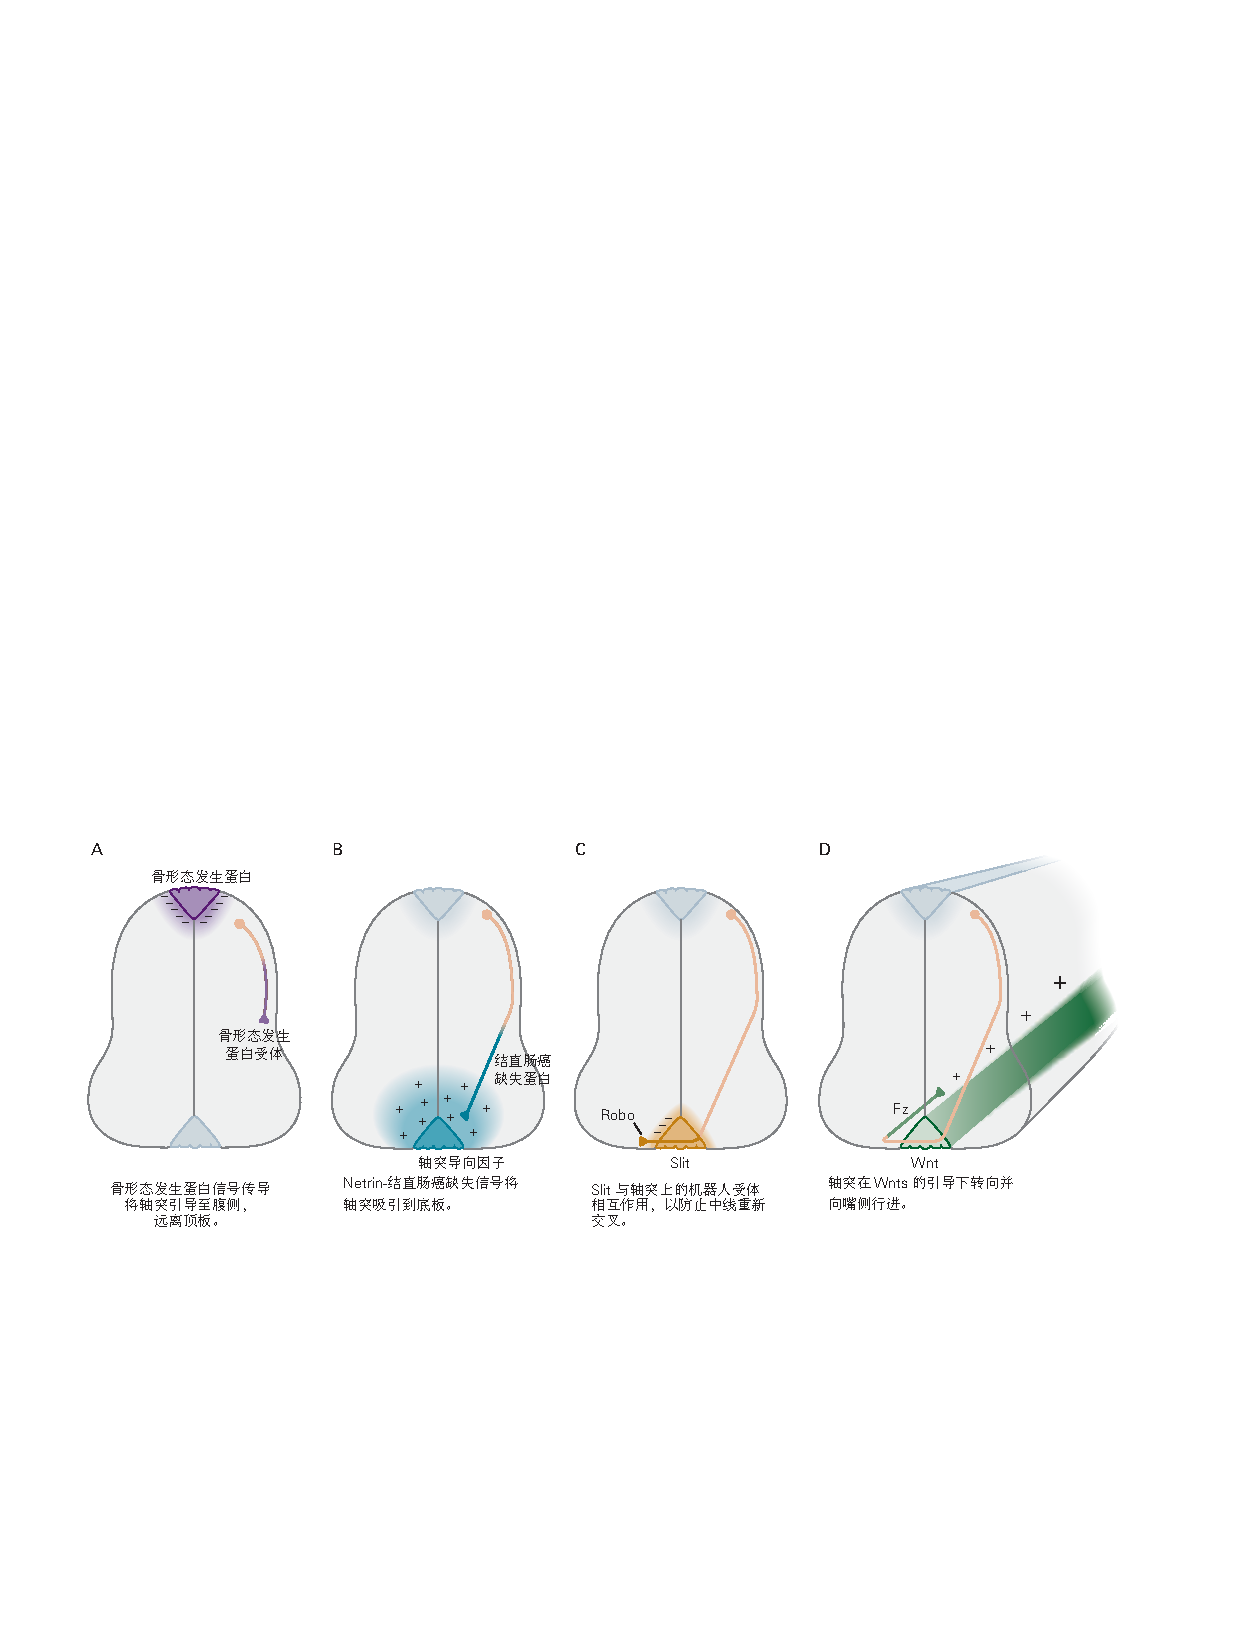
\includegraphics[width=1.0\linewidth]{chap47/fig_47_18}
	\caption{顶板和底板细胞表达的引导信号指导发育中脊髓中的连合轴突。
		A. 顶板细胞分泌的\textit{骨形态发生蛋白}与连合轴突上的\textit{骨形态发生蛋白受体}相互作用,以引导轴突远离顶板。
		B. 由底板细胞表达的\textit{轴突导向因子}将在\textit{结直肠癌缺失蛋白}中缺失的表达连合轴突吸引到脊髓的腹侧中线。
		\textit{音猬蛋白}也与连合轴突的腹侧引导有关。
		C. 底板细胞分泌的 Slit 蛋白与连合轴突上的 Robo 受体相互作用,以防止这些轴突再次穿过中线。
		在穿越之前,但不是之后,除了 robo1 和 robo2 之外,连合轴突还表达 robo3(Rig-1)。
		Rig-1 蛋白使 Robo 受体失活,防止轴突在靠近腹侧中线时对 Slits 的排斥作用做出反应。
		D. 连合轴突穿过中线后,底板细胞分泌的\textit{无翅型乳腺瘤病毒整合位点家族}蛋白以前后头尾梯度分布,并与连合轴突上的卷曲(Fz)蛋白相互作用,将轴突引向大脑。}
	\label{fig:47_18}
\end{figure}


最后,一旦轴突离开底板,它们就会转向大脑中最终的突触目标。
如图~\ref{fig:47_18}D~所示,底板细胞表达的\textit{无翅型乳腺瘤病毒整合位点家族}蛋白的头尾梯度似乎在腹侧中线处引导轴突向头部生长。
因此,在整个轴突发育过程的不同阶段,不同的信号指导连合轴突。
同样的过程可能会在数百甚至数千类神经元中进行,以建立成熟的大脑连接模式。



\section{要点}

1. 随着神经元延伸的进行,一个延伸通常变成轴突,其他延伸变成树突。
这个过程称为极化。
这两种类型的突起在结构、分子结构以及功能上有所不同。


2. 细胞类型在其树突的形状、大小和分支模式方面存在显著差异。
特定类型的树突特征既来自类型间转录程序的内在差异,也来自发育中的树突受到的外在影响。


3. 树突之间的相互作用对于树突的形成至关重要。
单个细胞的树突之间的排斥相互作用(称为自我回避的过程)导致区域的均匀覆盖,具有最小的间隙或团块。
相邻细胞树突之间的排斥作用(称为平铺的过程)可最大限度地减少树突区域的重叠。
在某些情况下,树突会避开其自身神经元的其他树突,但会与名义上相同的相邻细胞的树突相互作用。
这个过程称为自我/非自我辨别。


4. 轴突顶端的生长锥作为感觉和运动元件,引导轴突到达目的地。
生长锥的细胞骨架元素(包括肌动蛋白和肌球蛋白)促进生长。


5. 生长锥上的受体通过识别并结合轴突延伸所经过环境中的配体,从而引导生长。
这些相互作用导致它们第二信使的产生,这些第二信使介导生长锥的生长、转动和停止以及轴突分支的形成。


6. 一些生长锥包含蛋白质合成机器,包括\textit{信使核糖核酸}。
在这些情况下,受体可以促进介导生长或转变的特定蛋白质的局部合成。


7. 配体-受体对包括几个关键的分子家族,包括钙粘蛋白、Slits 及其Robo受体、\textit{信号素}及其神经丛蛋白受体,以及肝配蛋白及其 Eph 激酶受体。


8. 轴突向远处目标的生长被分解成离散的较短步骤。 
在每一步中,相邻结构表面的分子或由相邻结构分泌的分子都会引导轴突。
它们还可以导致生长锥的受体组成发生变化,使其能够在后续阶段对不同的信号做出反应。


9. \textit{罗杰$\cdot$斯佩里}提出了一个化学特异性假说来解释轴突从视网膜不同部位到视顶盖(上丘)不同部位的特定生长,形成有序的\textit{视网膜映射}。
肝配蛋白及其受体 Eph 激酶是指导映射形成的关键分子。
它们沿着视网膜和顶盖的表达分级,并且在很大程度上通过排斥不正确位置的轴突,而不是将它们吸引到正确的位置来起作用。


10. 吸引分子和排斥分子都引导轴突穿过中线结构,这一过程称为交叉。
进化上保守的信号包括Slits、\textit{轴突导向因子}和\textit{无翅型乳腺瘤病毒整合位点家族}。
编码这些配体和受体的基因突变可导致发育性神经系统疾病。

